\documentclass[11pt]{article}
\usepackage[a4paper, total={6.8in, 9.25in}]{geometry}
\usepackage{graphicx}
\graphicspath{ {./assets/images/output/} }
\usepackage{caption}
\usepackage[english]{babel}
\usepackage{titling}
\usepackage{float}
\usepackage{amsmath}
\usepackage{algorithm}
\usepackage{algorithmicx}
\usepackage{algpseudocode}
\usepackage{minted}
\usepackage{multicol}
\usepackage{array}
\usepackage{setspace}
\usepackage{placeins}
\usepackage{tcolorbox}
\usepackage{caption}
\usepackage{subcaption}

\definecolor{verbgray}{gray}{.95}
\setminted{
    bgcolor=verbgray,
    baselinestretch=1,
    fontsize=\footnotesize,
    linenos,
    breaklines=true,
    breakanywhere=true,
    xleftmargin=\parindent
}
\title{Implementation of Linear and Logistic Regression for Regression and Classification Problems}
\author{}
\date{}

\pagenumbering{gobble}
\begin{document}
\input{ml_cover.tex}

\pagebreak

\tableofcontents

\pagebreak
\pagenumbering{arabic}
\maketitle

\section{Theory and Introduction}
Linear Regression and Logistic Regression are fundamental algorithms in supervised machine learning. Linear Regression attempts to model the relationship between a scalar response and one or more explanatory variables by fitting a linear equation to observed data \cite{bishop2006pattern}. The objective is to minimize the difference between the predicted value and the actual value, typically quantified by the Mean Squared Error (MSE).

Logistic Regression, despite its name, is a classification algorithm used to estimate the probability that a given instance belongs to a particular class. It transforms the output of a linear equation using the Sigmoid function, mapping predictions to a probability range between 0 and 1 \cite{hastie2009elements}. The cost function used is the Log Loss (Binary Cross-Entropy), which is convex and suitable for gradient-based optimization.

In this experiment, both algorithms were implemented using Python (NumPy and Pandas) and applied to both problem domains (regression and classification) to observe their behavior and limitations.

\section{Methodology}
The implementation was divided into four distinct tasks. For all tasks, the dataset was split into training (80\%) and testing (20\%) sets. Feature scaling (Standardization) was applied where necessary to ensure convergence of Gradient Descent.

\subsection{Datasets Used}
Two primary datasets were selected to evaluate the models:
\begin{itemize}
    \item \textbf{Regression Dataset (Housing Data):} The \textit{California Housing} dataset was utilized to test the regression capabilities of the algorithms. This dataset contains metrics such as median income and house age to predict median house values \cite{pace1997sparse}.
    \item \textbf{Classification Dataset (Iris):} The standard \textit{Iris} dataset was used for classification tasks. To ensure binary classification, the dataset was filtered to include only two species: \textit{Versicolor} and \textit{Virginica} \cite{fisher1936use}.
\end{itemize}

\subsection{Algorithms Implemented}

\subsubsection{Task 1: Linear Regression (Regression Problem)}
This model was implemented to predict continuous values. The cost function $J(\theta)$ was minimized using Gradient Descent.

\begin{algorithm}[H]
    \caption{Linear Regression (Gradient Descent)}
    \begin{algorithmic}[1]
        \State \textbf{Input:} $X$ (Features), $y$ (Target), $\alpha$ (Learning Rate), $N$ (Iterations)
        \State \textbf{Initialize:} Weights $\theta \gets \vec{0}$, Bias added to $X$
        \For{$i = 1$ to $N$}
        \State $\hat{y} \gets X \cdot \theta$ \Comment{Linear Hypothesis}
        \State $error \gets \hat{y} - y$
        \State $gradient \gets \frac{1}{m} X^T \cdot error$
        \State $\theta \gets \theta - \alpha \cdot gradient$ \Comment{Update Rule}
        \State $J(\theta) \gets \frac{1}{2m} \sum (\hat{y} - y)^2$ \Comment{Compute MSE Cost}
        \EndFor
        \State \textbf{Output:} Optimized $\theta$
    \end{algorithmic}
\end{algorithm}

\begin{multicols}{2}
    \inputminted{python}{assets/1_linReg_reg.py}
\end{multicols}

\subsubsection{Task 2: Linear Regression (Classification Problem)}
Linear Regression was adapted for classification by applying a threshold to the continuous output.

\begin{algorithm}[H]
    \caption{Linear Regression for Classification}
    \begin{algorithmic}[1]
        \State \textbf{Train:} Run \textit{Linear Regression (Gradient Descent)} to find $\theta$
        \State \textbf{Predict:}
        \For{each sample $x$ in $X_{test}$}
        \State $\hat{y}_{raw} \gets x \cdot \theta$
        \If{$\hat{y}_{raw} \geq 0.5$}
        \State $\hat{y}_{class} \gets 1$
        \Else
        \State $\hat{y}_{class} \gets 0$
        \EndIf
        \EndFor
        \State \textbf{Evaluate:} Compare $\hat{y}_{class}$ with true labels.
    \end{algorithmic}
\end{algorithm}

\begin{multicols}{2}
    Only the classification-specific code is shown here.
    \inputminted{python}{assets/2_linReg_cls.py}
\end{multicols}

\subsubsection{Task 3: Logistic Regression (Regression Problem)}
Since Logistic Regression is a classifier, the regression target (e.g., House Price) was converted into a binary target (High vs. Low Value) based on the median price.

\begin{algorithm}[H]
    \caption{Logistic Regression (Target Transformation)}
    \begin{algorithmic}[1]
        \State \textbf{Pre-processing:}
        \State $median \gets Median(y_{continuous})$
        \State $y_{binary} \gets [1 \text{ if } y_i > median \text{ else } 0 \text{ for } y_i \text{ in } y]$
        \State \textbf{Train:} Run \textit{Logistic Regression} on $(X, y_{binary})$
        \State \textbf{Evaluate:} Classification metrics (Accuracy, F1) on the binned target.
    \end{algorithmic}
\end{algorithm}

\begin{multicols}{2}
    Only the target transformation code is shown here.
    \inputminted{python}{assets/3_logReg_reg.py}
\end{multicols}

\subsubsection{Task 4: Logistic Regression (Classification Problem)}
The standard implementation using the Sigmoid activation function and Log Loss cost.

\begin{algorithm}[H]
    \caption{Logistic Regression (Standard)}
    \begin{algorithmic}[1]
        \State \textbf{Input:} $X$, $y$, $\alpha$, $N$
        \State \textbf{Function:} $h_\theta(x) = \frac{1}{1 + e^{-X\theta}}$
        \For{$i = 1$ to $N$}
        \State $z \gets X \cdot \theta$
        \State $\hat{y} \gets \sigma(z)$ \Comment{Sigmoid Activation}
        \State $gradient \gets \frac{1}{m} X^T \cdot (\hat{y} - y)$
        \State $\theta \gets \theta - \alpha \cdot gradient$
        \State $Cost \gets -\frac{1}{m} \sum [y \log(\hat{y}) + (1-y) \log(1-\hat{y})]$
        \EndFor
    \end{algorithmic}
\end{algorithm}

\begin{multicols}{2}
    \inputminted{python}{assets/4_logReg_cls.py}
\end{multicols}

\section{Results and Discussion}

\subsection{Linear Regression Results}

\subsubsection{Task 1: Regression on Continuous Data}
The Linear Regression model was applied to the regression dataset to predict continuous outcomes. The training process was initialized with a learning rate of 0.01 for 1000 iterations. The model parameters converged to weights of $\theta = [22997.42, 9768.48]$, indicating a bias term of approximately 22,997 and a feature coefficient of 9,768.

\begin{minted}{console}
Training Linear Regression (LR=0.01, Iter=1000)...

========================================
EVALUATION REPORT
========================================
Final Weights (Theta): [22997.42197203  9768.48083188]
Mean Squared Error (MSE): 52,876,610.79
R2 Score (Accuracy):      0.8965
(Confusion Matrix / ROC are not applicable to Regression)
\end{minted}

An $R^2$ score of 0.8965 suggests that approximately 89.65\% of the variance in the target variable is explained by the model. As observed in Figure \ref{fig:lin_reg_task1}, the cost function decreased rapidly, and the regression line demonstrates a strong fit to the data points. The console output is as follows:

\begin{figure}[H]
    \centering
    % REPLACE WITH YOUR IMAGE FILENAME
    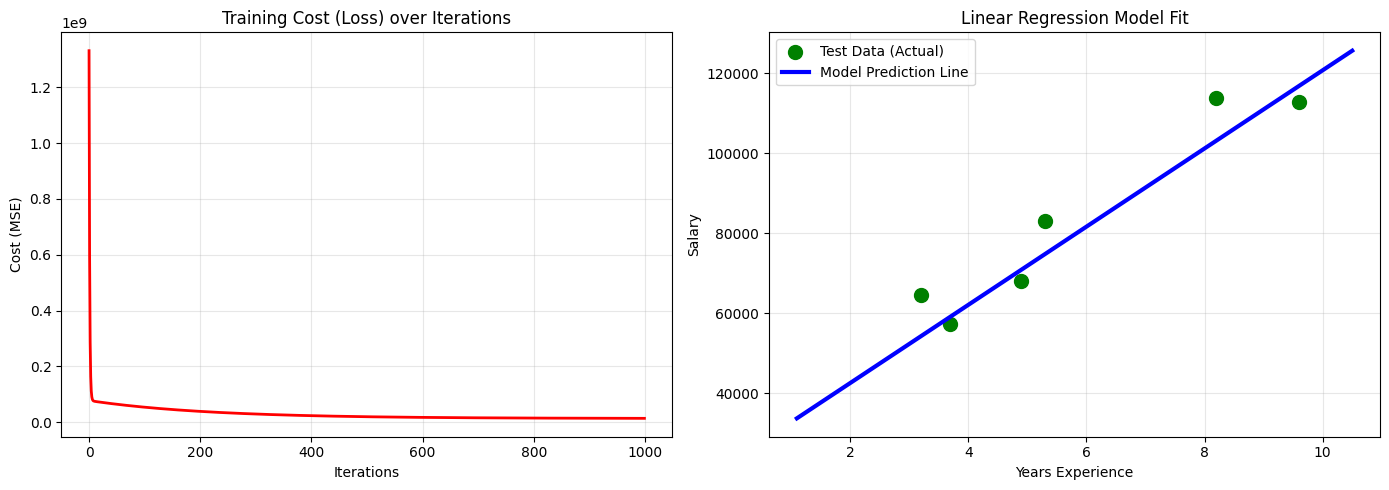
\includegraphics[width=1.0\textwidth]{task1_training_fit.png}
    \caption{Task 1 Evaluation: Training Cost history (Left) and Linear Model Fit (Right).}
    \label{fig:lin_reg_task1}
\end{figure}

\subsubsection{Task 2: Linear Regression on Classification Data}
The Linear Regression algorithm was experimentally applied to the Iris classification task by using a decision threshold of 0.5 on the predicted continuous values. Despite the algorithm being designed for regression, it achieved high accuracy on this linearly separable subset of the data. The console output is as follows:

\begin{minted}{console}
Dataset loaded successfully!
Training Linear Regression on Classification Data...

========================================
EVALUATION REPORT
========================================
Algorithm: Linear Regression (MSE) applied to Classification
Threshold: 0.5
----------------------------------------
Accuracy:  0.9500
Precision: 1.0000
Recall:    0.8750
F1 Score:  0.9333

Confusion Matrix:
      Pred 0  Pred 1
Act 0   12       0
Act 1   1       7    
\end{minted}

The confusion matrix indicates that while the precision was perfect (no False Positives), there was one False Negative (Recall of 0.875), resulting in a slight drop in the F1 score. Figure \ref{fig:lin_reg_class} illustrates the ROC curve and the decision boundary established by the linear function.

\begin{figure}[H]
    \centering
    % REPLACE WITH YOUR IMAGE FILENAME
    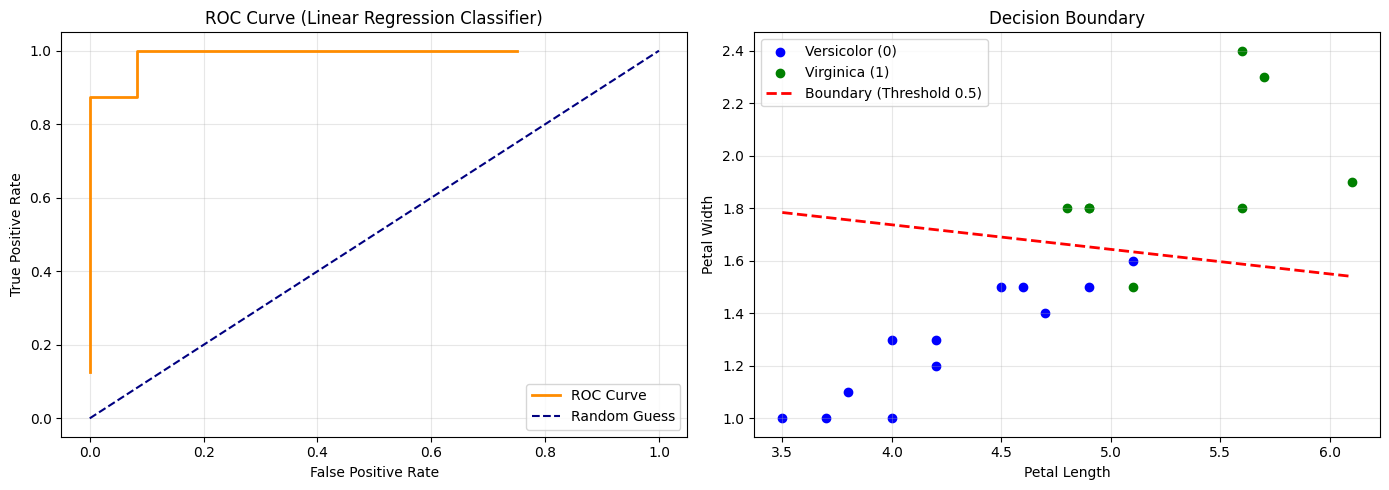
\includegraphics[width=1.0\textwidth]{task2_roc_boundary.png}
    \caption{Task 2 Evaluation: ROC Curve (Left) and Decision Boundary (Right).}
    \label{fig:lin_reg_class}
\end{figure}

\subsection{Logistic Regression Results}

\subsubsection{Task 3: Logistic Regression on Regression Data}
To apply Logistic Regression to the Housing dataset, the continuous target was transformed into a binary classification problem. The median house price was calculated as \$181,600. Houses priced above this median were labeled "High Value," and those below or equal were labeled "Low Value."

\begin{minted}{console}
Median House Price: $181,600
Task: Predict if House Price is > Median (High Value) or <= Median (Low Value)
Training Logistic Regression on Housing Data...

========================================
EVALUATION REPORT (Housing Data)
========================================
Accuracy:  80.00%
Precision: 79.17%
Recall:    79.17%
F1 Score:  0.7917
--------------------
Confusion Matrix:
[[84 20]
 [20 76]]
\end{minted}

The model achieved an accuracy of 80\%, with the confusion matrix showing a balanced distribution of errors (20 False Positives and 20 False Negatives). Figure \ref{fig:log_reg_housing} displays the cost reduction, the decision boundary separating high and low-value regions, and the resulting confusion matrix.

\begin{figure}[H]
    \centering
    % REPLACE WITH YOUR IMAGE FILENAME
    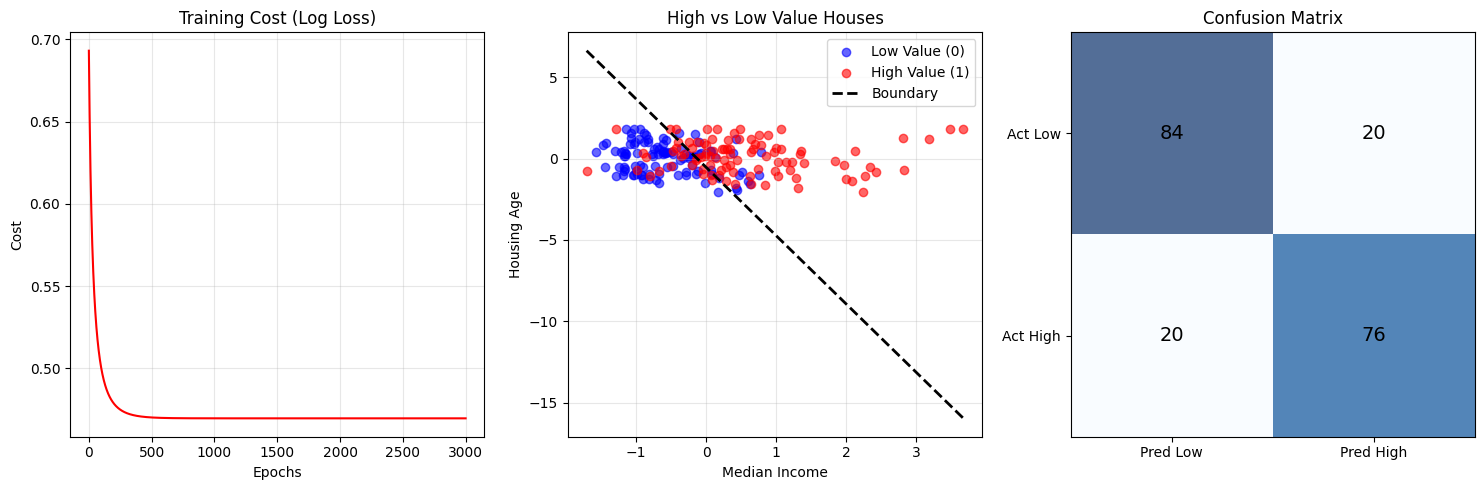
\includegraphics[width=1.0\textwidth]{task3_cost_boundary_cm.png}
    \caption{Task 3 Evaluation: Training Cost (Left), Decision Boundary for High/Low Price (Middle), and Confusion Matrix (Right).}
    \label{fig:log_reg_housing}
\end{figure}

\subsubsection{Task 4: Logistic Regression on Classification Data}
Finally, the standard Logistic Regression model was tested on the binary Iris dataset (100 samples). The model converged successfully, providing probabilistic classification predictions.


\begin{minted}{console}
Dataset Size: 100 samples (Versicolor & Virginica)
Training Logistic Regression...

========================================
LOGISTIC REGRESSION REPORT
========================================
Accuracy:  90.00%
Precision: 87.50%
Recall:    87.50%
F1 Score:  0.8750
--------------------
Confusion Matrix:
[[11  1]
 [ 1  7]]
\end{minted}

The confusion matrix reveals two misclassifications (one False Positive and one False Negative) out of the test set, resulting in an accuracy of 90\%. Figure \ref{fig:log_reg_iris} provides a comprehensive view of the model's performance, including the cost history, ROC curve, confusion matrix, and the decision boundary relative to the data points.

\begin{figure}[H]
    \centering
    % REPLACE WITH YOUR IMAGE FILENAME
    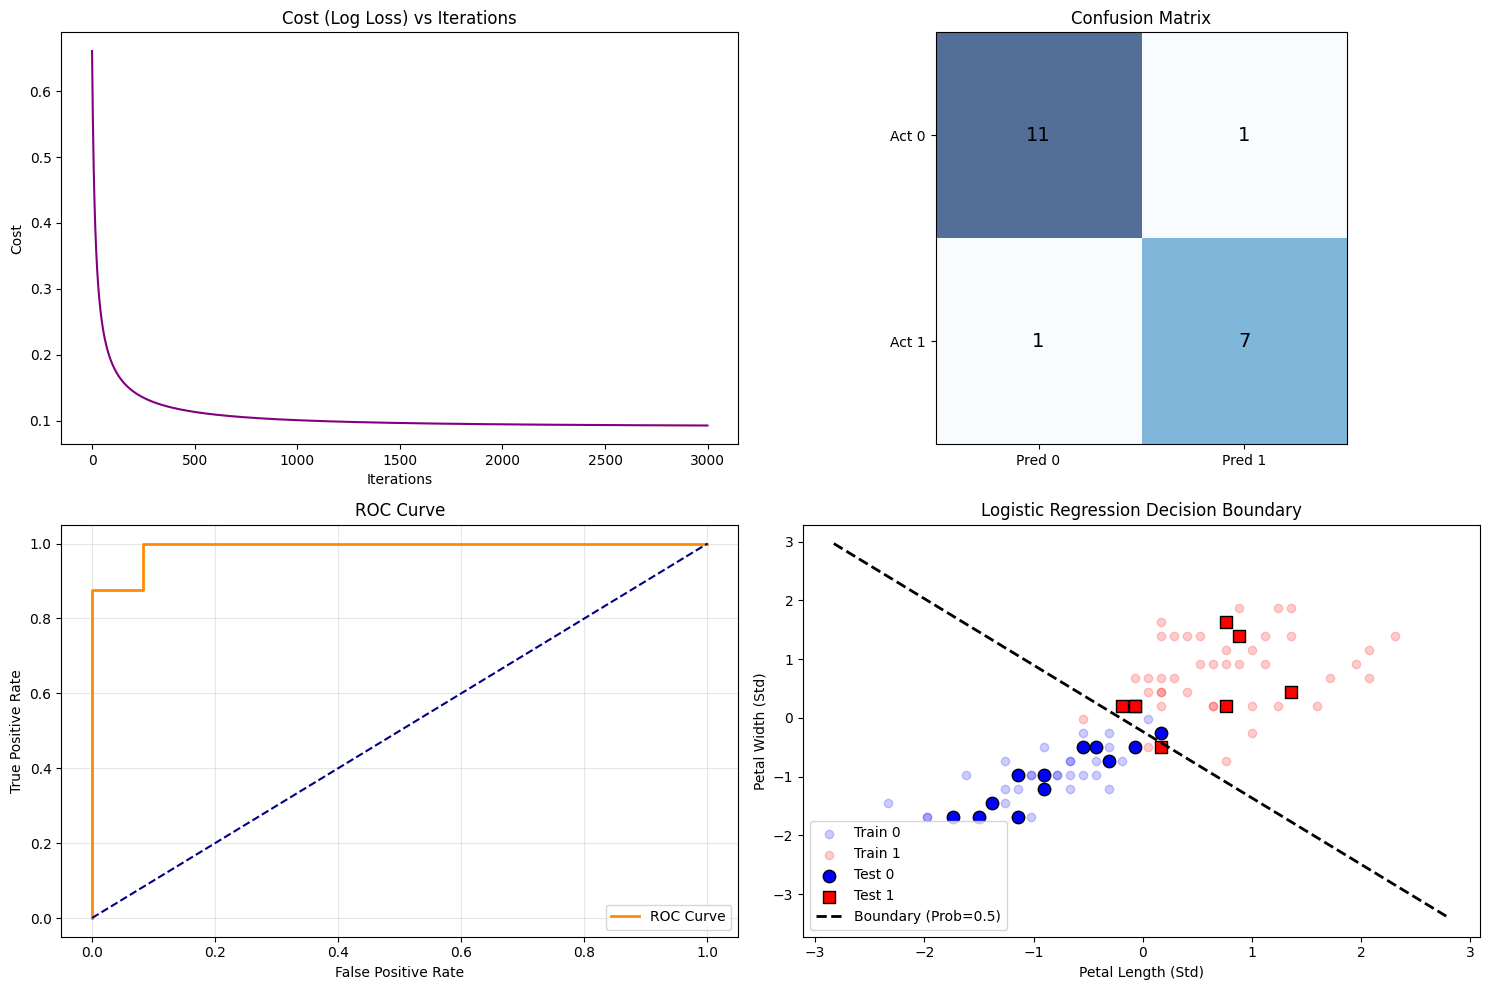
\includegraphics[width=.9\textwidth]{task4_quad_plot.png}
    \caption{Task 4 Evaluation: Training Cost (Top-Left), Confusion Matrix (Top-Right), ROC Curve (Bottom-Left), and Decision Boundary (Bottom-Right).}
    \label{fig:log_reg_iris}
\end{figure}

\section{Conclusion}
In this sessional, Linear and Logistic Regression algorithms were implemented from scratch and evaluated across different domains. Linear Regression proved highly effective for the regression task, achieving an $R^2$ score of 0.8965. When forced into a classification role (Task 2), it performed surprisingly well (95\% accuracy) but remains theoretically suboptimal due to its sensitivity to outliers and unbounded output. Logistic Regression demonstrated robust performance on the standard classification task (90\% accuracy). When adapted for regression data via binning (Task 3), it provided a viable method for coarse-grained prediction (High vs. Low value), achieving 80\% accuracy. The successful convergence of the cost functions in all four tasks confirms the correctness of the Gradient Descent implementation.


\bibliographystyle{IEEEtran}
\renewcommand{\bibname}{References}
\addcontentsline{toc}{section}{References}
\bibliography{ref}

\end{document}
